\section{Auswertung zum Shinriki-Oszillator}

\subsection{Phasendiagramm}
Im Folgenden wurde ein Phasendiagramm des Shinrinki-Oszillators mit den Werten \(R_1\) und \(R_2\) erstellt. Dafür wurden Schnittpunkte der Phasenübergänge ermittelt und mithilfe eines Python-Skripts wurde diese Punkte mit einer Funktion verbunden. Daraus ergibt sich folgende Abbildung, welche die Übergänge der verschiedenen Phasen abhängig von den Werten der Widerstände darstellen. Jede Line stellt dabei einen Phasenübergang dar.

\begin{figure}[h]
    \centering
    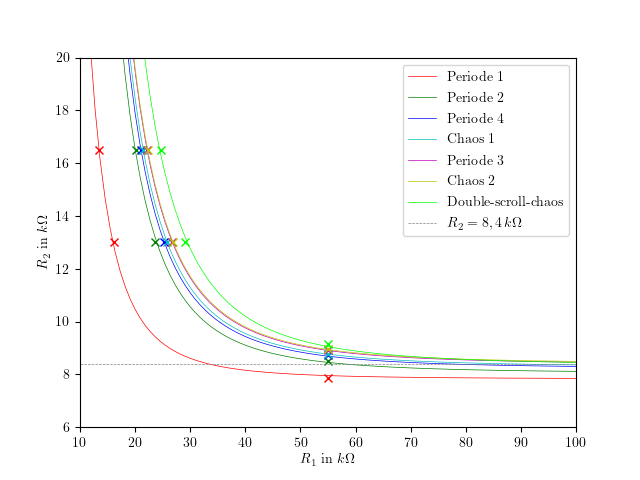
\includegraphics[scale=0.75]{AuswPaul/PhasendiagrammFertig.png}
    \label{fig:Phasendiagramm}
    \caption{Phasendiagramm}
\end{figure}

Die Funktion welche benutzt wurde, um die Punkte zu verbinden ist:
\begin{align}
    f = \frac{a}{x^3} +b
\end{align}

Hier: $R_1 = f$, $R_2 = x$ und $R_0 = b$.


Diese Funktion wurde ausgewählt, indem mehrere verschiedene Funktionen ausprobiert wurden. Nachfolgend ausgewählte Funktionen zum Vergleich, um die Auswahl nachvollziehen zu können.
\begin{figure}[h]

    \centering
    
    \begin{subfigure}[b]{0.45\textwidth}
        \centering
        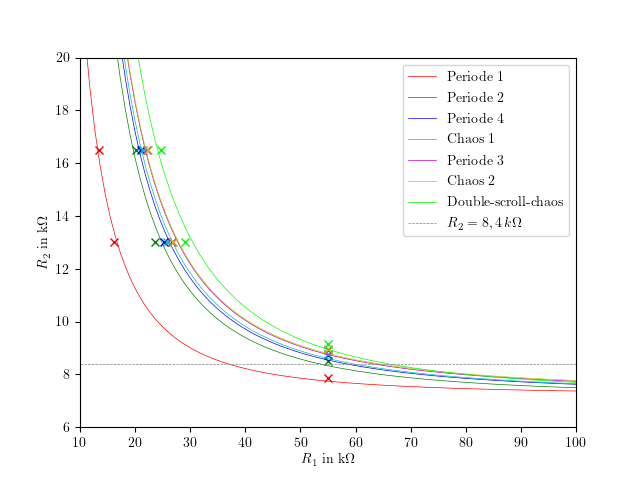
\includegraphics[width=\textwidth]{AuswPaul/PhaDiaGrad-2.png}
        \caption{$f = \frac{a}{x^2} + b$}
    \end{subfigure}
    \hfill
    \begin{subfigure}[b]{0.45\textwidth}
        \centering
        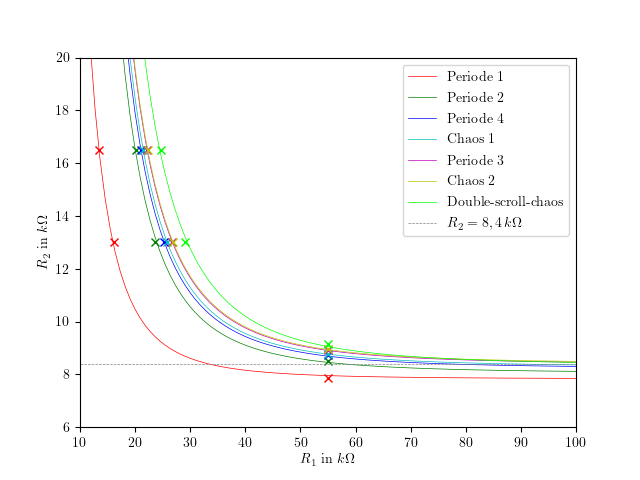
\includegraphics[width=\textwidth]{AuswPaul/PhasendiagrammFertig.png}
        \caption{$f = \frac{a}{x^3} + b$}
    \end{subfigure}
    \\
    \begin{subfigure}[b]{0.45\textwidth}
        \centering
        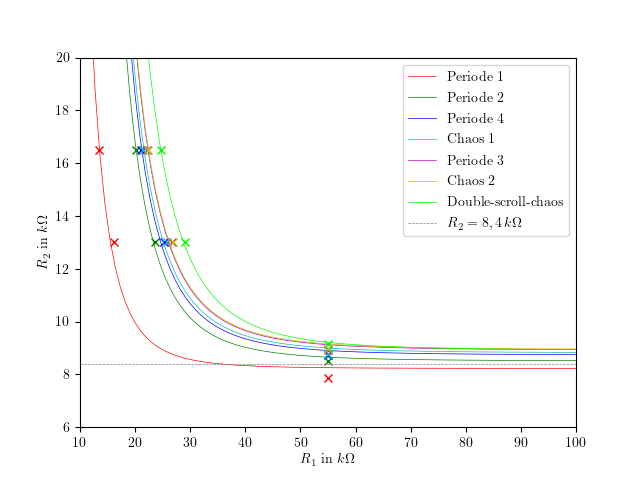
\includegraphics[width=\textwidth]{AuswPaul/PhaDiaGrad-4.png}
        \caption{$f = \frac{a}{x^4} + b$}
    \end{subfigure}
    \caption{Vergleich verschiedener 'Fitting'-Funktionen}
    \label{fig:PhasenDiaVergl}
    \end{figure}\\
\newpage
Anbei noch die errechneten Parameter für die einzelnen Funktionen: \\
\begin{table}[h]
    \centering
    \begin{tabular}{l|r|r}
            Übergang auf &     a in Ohm$^4$ & b in Ohm\\
            \hline
               Periode 1 &   21098,64 &  7,83 \\
               Periode 2 &   67878,80 &  8,05 \\
               Periode 4 &   77374,66 &  8,23 \\
                 Chaos 1 &   81341,62 &  8,28 \\
               Periode 3 &   88743,91 &  8,37 \\
                 Chaos 2 &   89540,79 &  8,40 \\
     Double-scroll-chaos &  119710,19 &  8,33 \\
    \end{tabular}
    \caption{Fitting-Parameter}
\end{table}



\subsection{Schnitt durch das Phasendiagramm}
Nun wird für einen festen Wert (\(R_2 = 8,4 k\Omega\)) ein Schnitt durch das Phasendiagramm erzeugt, indem \(R_1\) variiert wird und die Veränderungen aufmerksam beobachtet werden. \\
Im Folgenden unsere Beobachtungen bei ausgewählten Werten von \(R_1\).\\

\begin{figure}[h]
    \centering
    \begin{subfigure}[b]{0.45\textwidth}
        \centering
        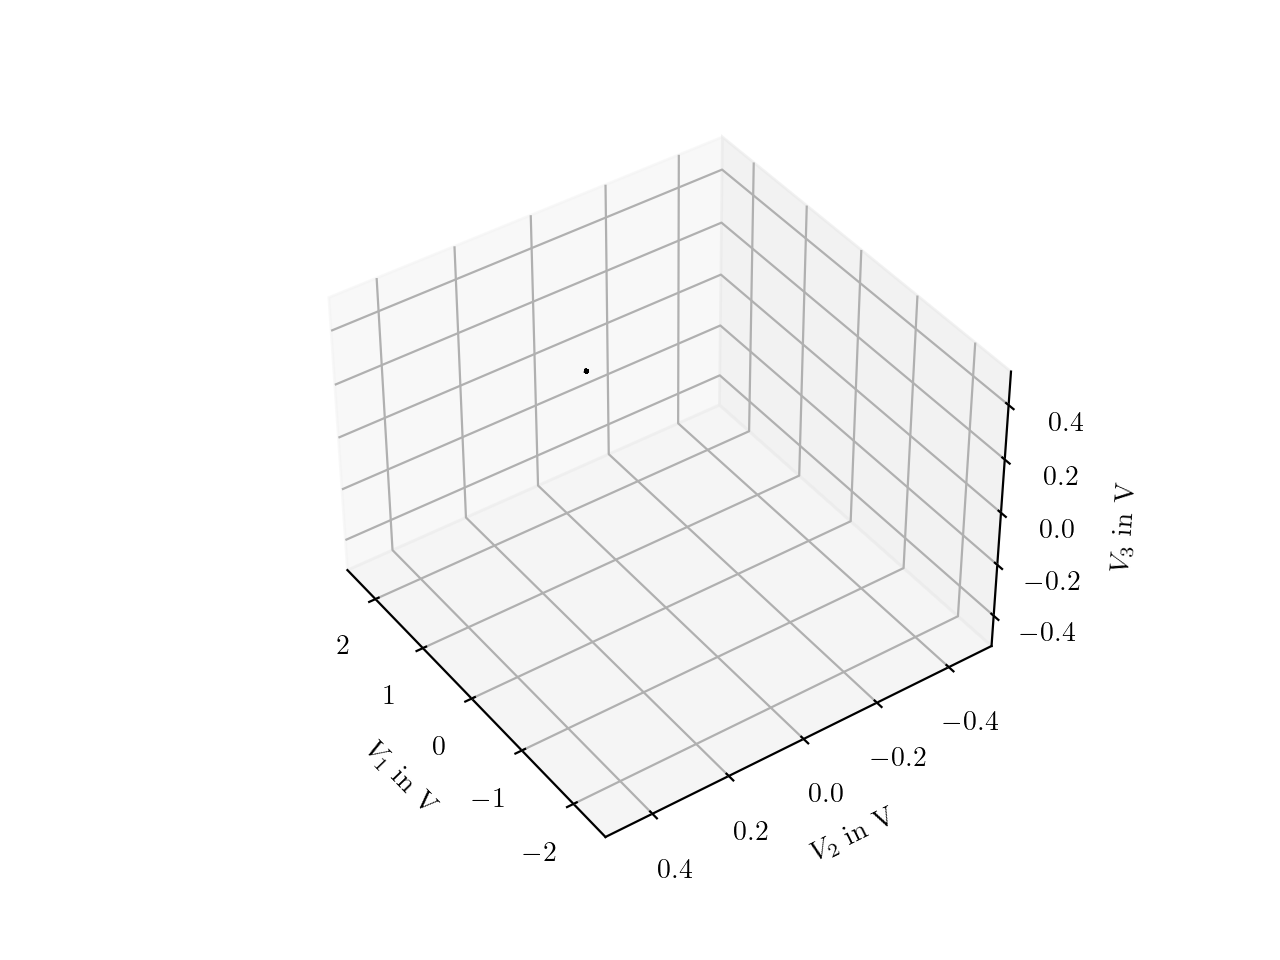
\includegraphics[width=\textwidth]{AuswPaul/Aufg-b/At37.png}
        \caption{Attraktor}
    \end{subfigure}
    \hfill
    \begin{subfigure}[b]{0.45\textwidth}
        \centering
        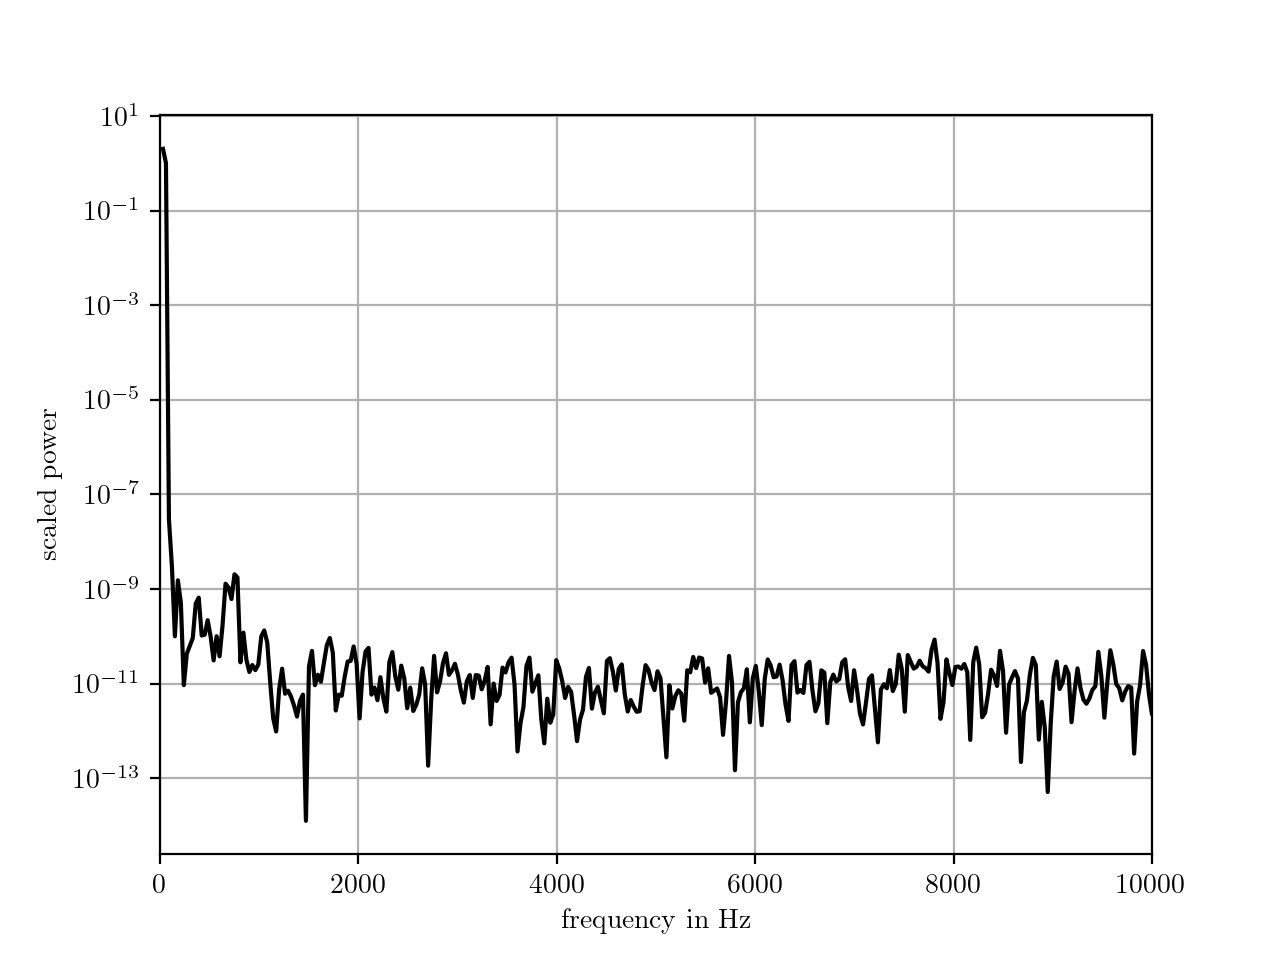
\includegraphics[width=\textwidth]{AuswPaul/Aufg-b/LS37.png}
        \caption{Leistungsspektrum}
    \end{subfigure}
    \caption{$R_1 = 37$ k$\Omega$}
    \label{fig:A37}
\end{figure}

Bei $R_1 = 37$ k$\Omega$ (Abbildung \ref{fig:A37}) ist anhand des Attraktors zu erkennen, dass keine Schwingung auftritt. Auch das Leistungsspektrum verläuft, bis auf einen Peak bei ca. 0 Hz erstaunlich gleichmäßig und bis auf Störungsrauschen nahezu horizontal. Dies spricht ebenfalls für ein schwingungsfreies System.\\

\begin{figure}[h]
    \centering
    \begin{subfigure}[b]{0.45\textwidth}
        \centering
        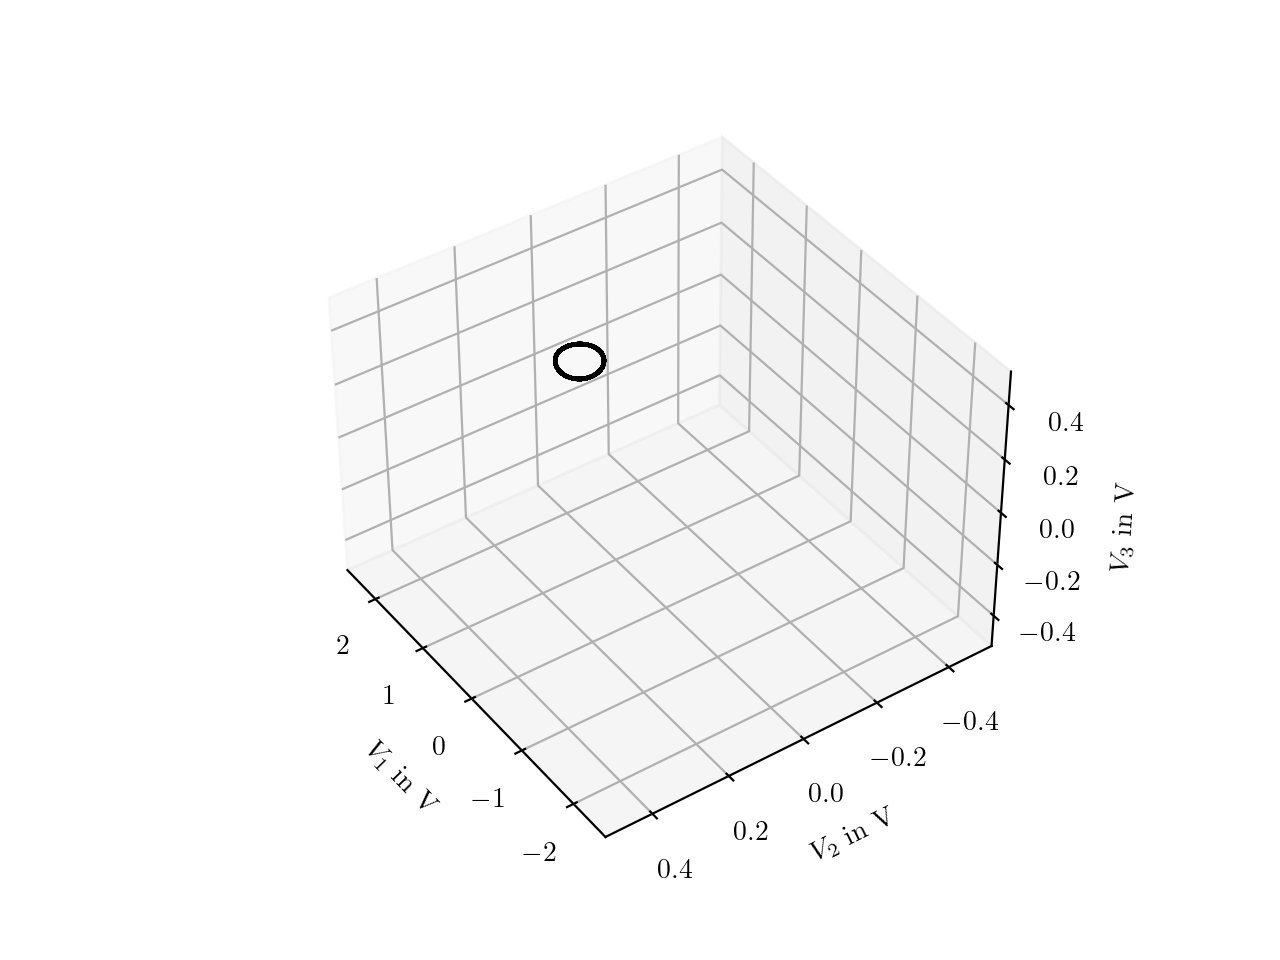
\includegraphics[width=\textwidth]{AuswPaul/Aufg-b/At40.png}
        \caption{Attraktor}
    \end{subfigure}
    \hfill
    \begin{subfigure}[b]{0.45\textwidth}
        \centering
        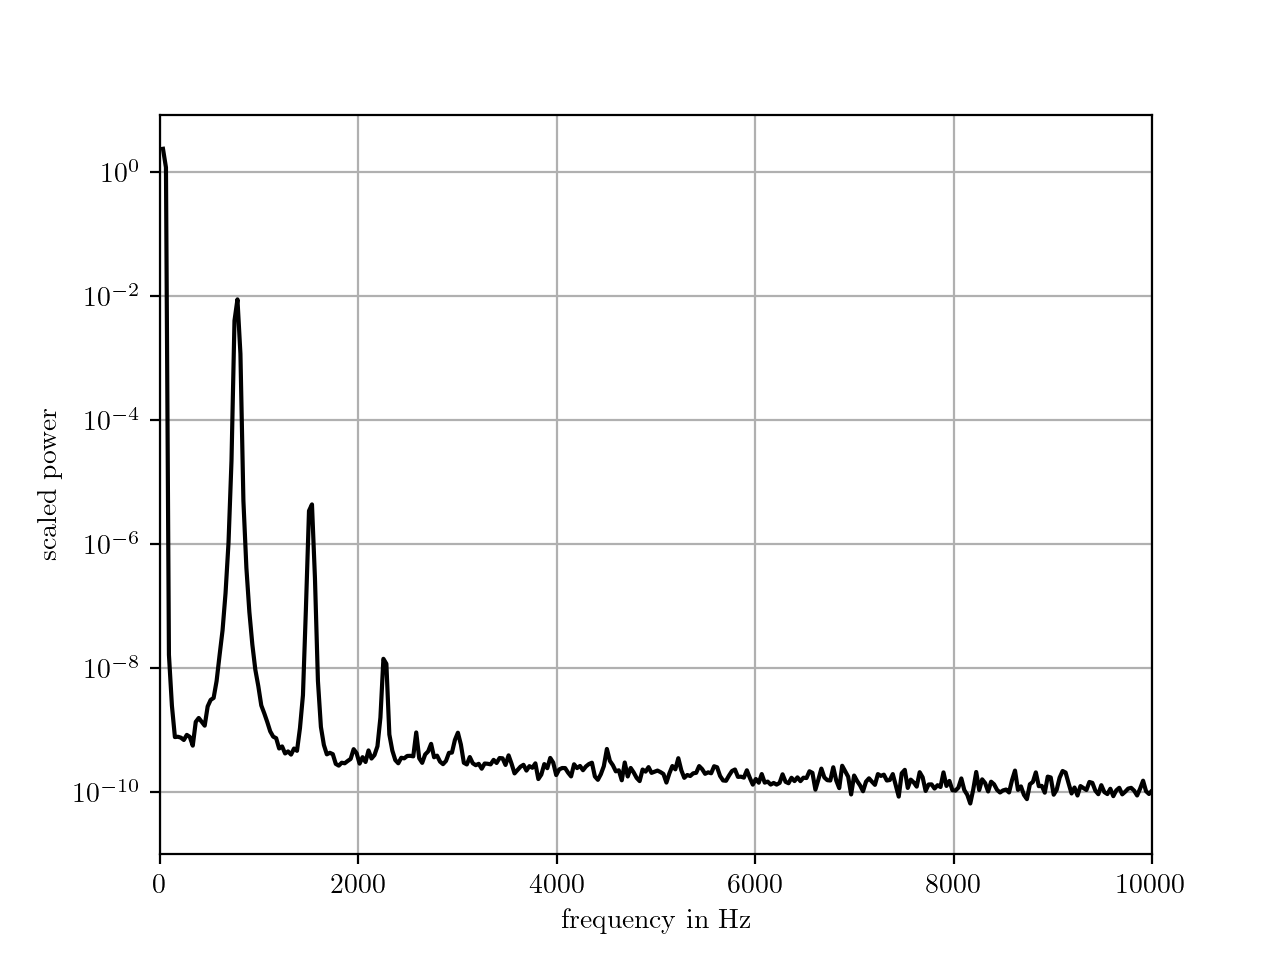
\includegraphics[width=\textwidth]{AuswPaul/Aufg-b/LS40.png}
        \caption{Leistungsspektrum}
    \end{subfigure}
    \caption{$R_1 = 40$ k$\Omega$}
    \label{fig:A40}
\end{figure}

Für $R_1 =40$ k$\Omega$ (Abbildung \ref{fig:A40}) befindet sich der Shinriki-Oszilator bereits in Periode 1, was deutlich anhand des Attraktors zu erkennen ist. Auch im Leistungsspektrum sind nun deutliche Unterschiede im Vergleich zum voran gegangenen zu erkennen. Es ist nun die erste Grundschwingung und die 1. harmonische zu erkennen.

\begin{figure}[h]
    \centering
    \begin{subfigure}[b]{0.45\textwidth}
        \centering
        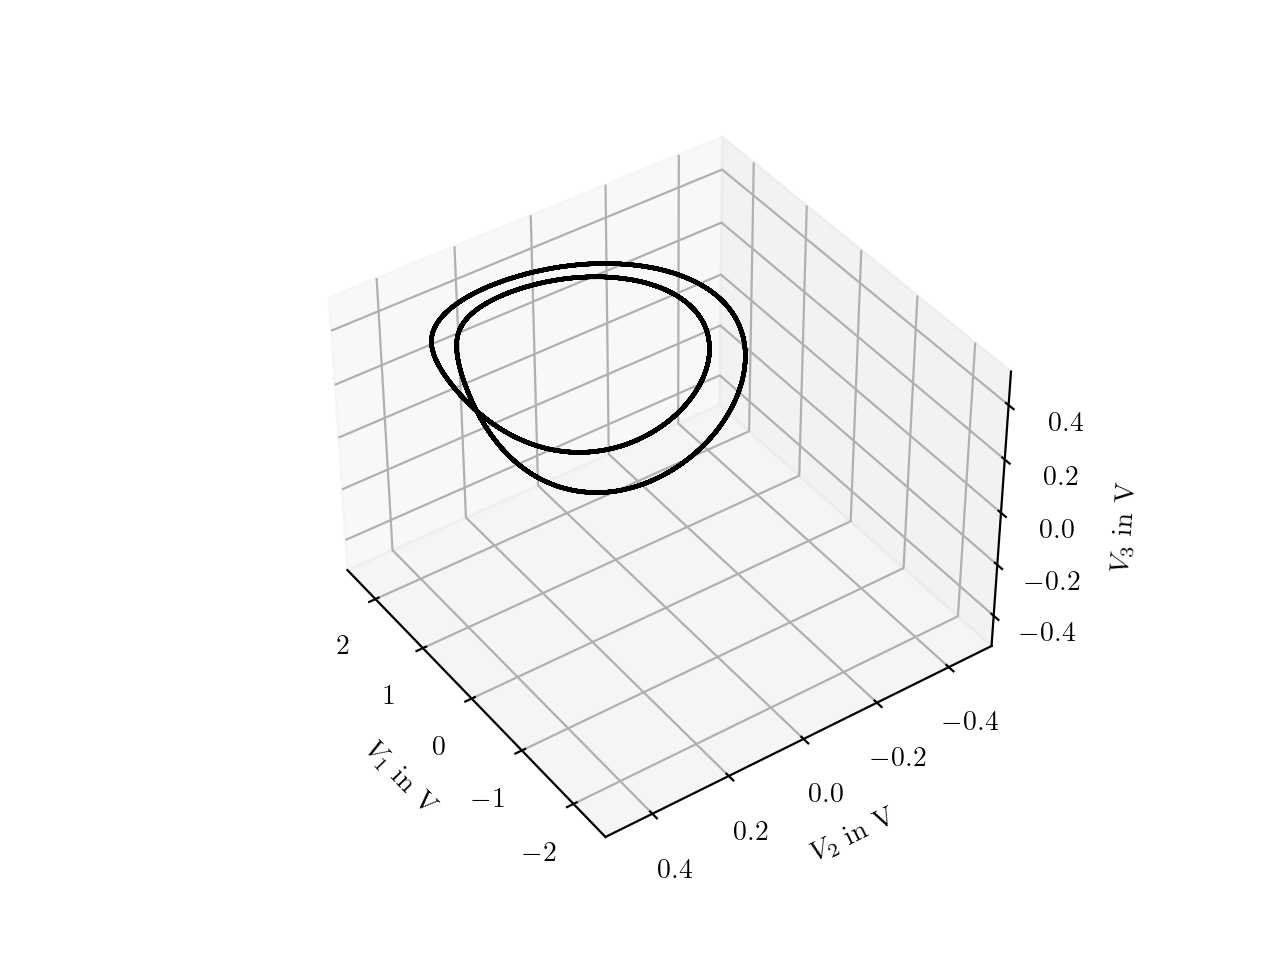
\includegraphics[width=\textwidth]{AuswPaul/Aufg-b/At60.png}
        \caption{Attraktor}
    \end{subfigure}
    \hfill
    \begin{subfigure}[b]{0.45\textwidth}
        \centering
        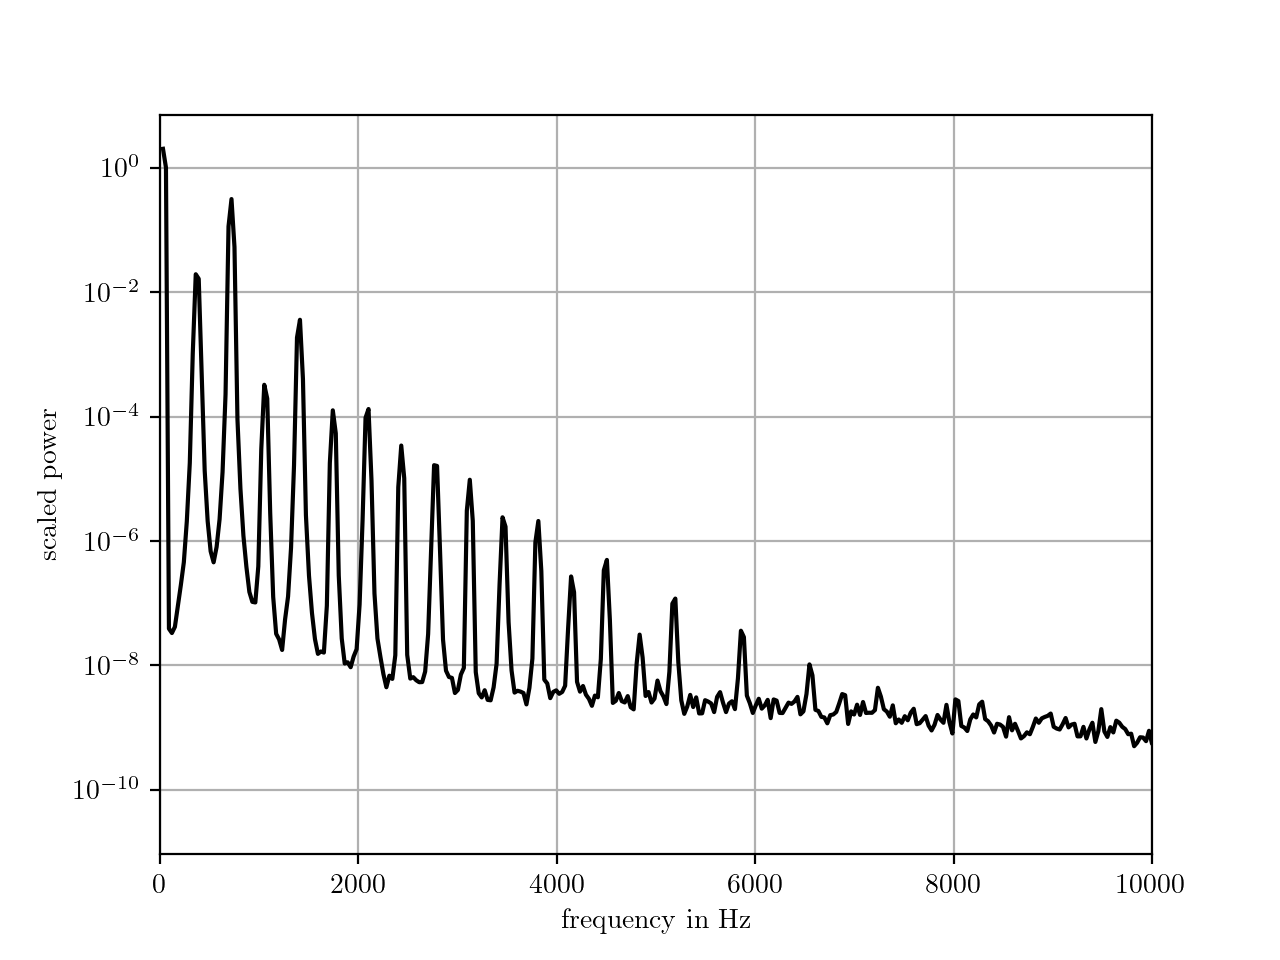
\includegraphics[width=\textwidth]{AuswPaul/Aufg-b/LS60.png}
        \caption{Leistungsspektrum}
    \end{subfigure}
    \caption{$R_1 = 60$ k$\Omega$}
    \label{fig:A60}
\end{figure}

Eine deutliche Zunahme an Peaks ist bei $R_1 = 60$ k$\Omega$ (Abbildung \ref{fig:A60}) zu erkennen. Nun ist eine subharmonische Schwinung mit $\frac{1}{2} f_0$ zu erkennen. Anhand des Attraktors ist sehr gut zu erkennen, dass es sich nun um Periode 2 handelt. Im Vergleich zum letzten Mal fand also ein Bifurkation statt.

\begin{figure}[h]
    \centering
    \begin{subfigure}[b]{0.45\textwidth}
        \centering
        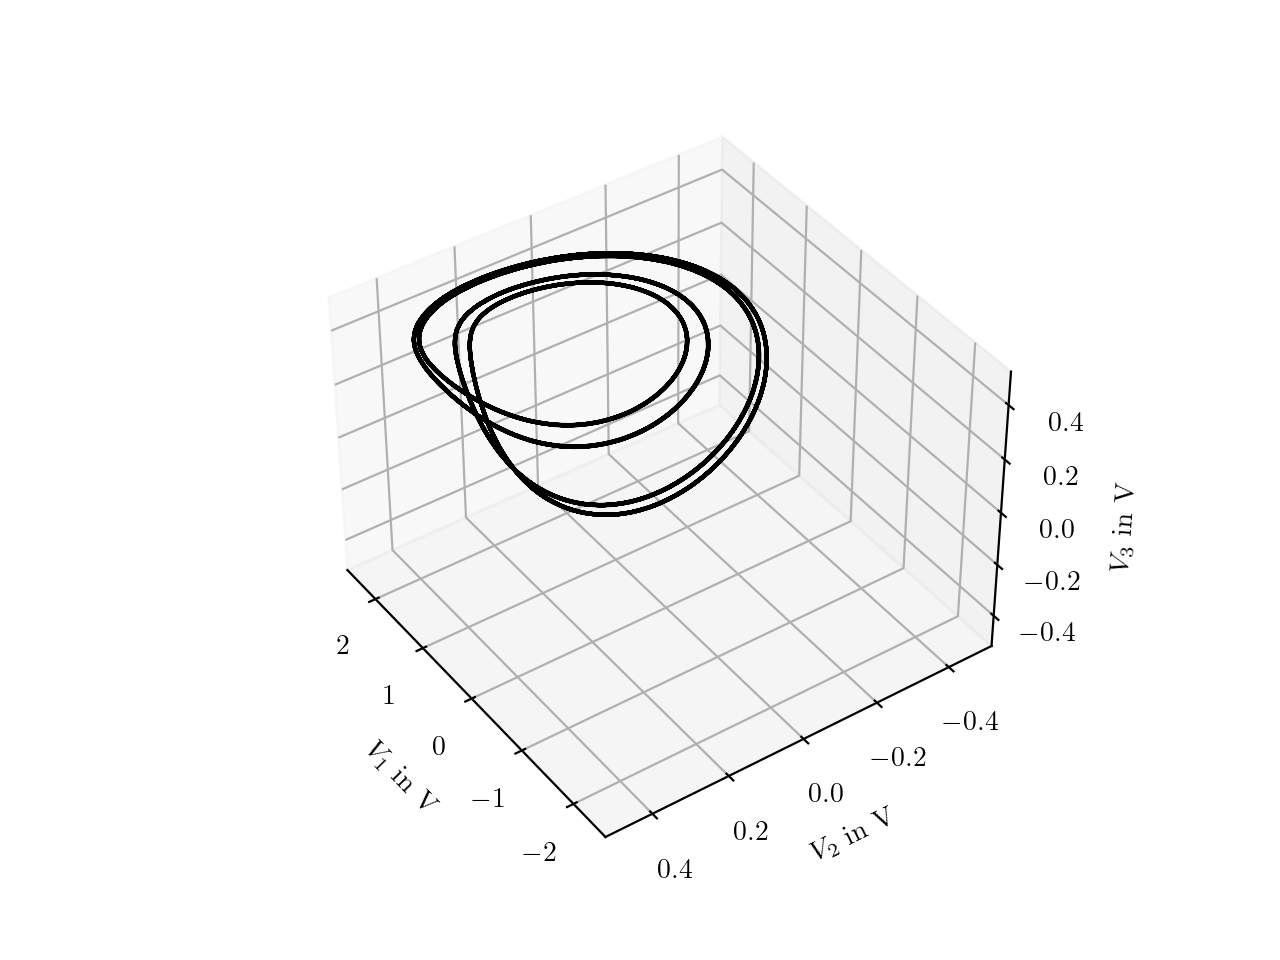
\includegraphics[width=\textwidth]{AuswPaul/Aufg-b/At66.png}
        \caption{Attraktor}
    \end{subfigure}
    \hfill
    \begin{subfigure}[b]{0.45\textwidth}
        \centering
        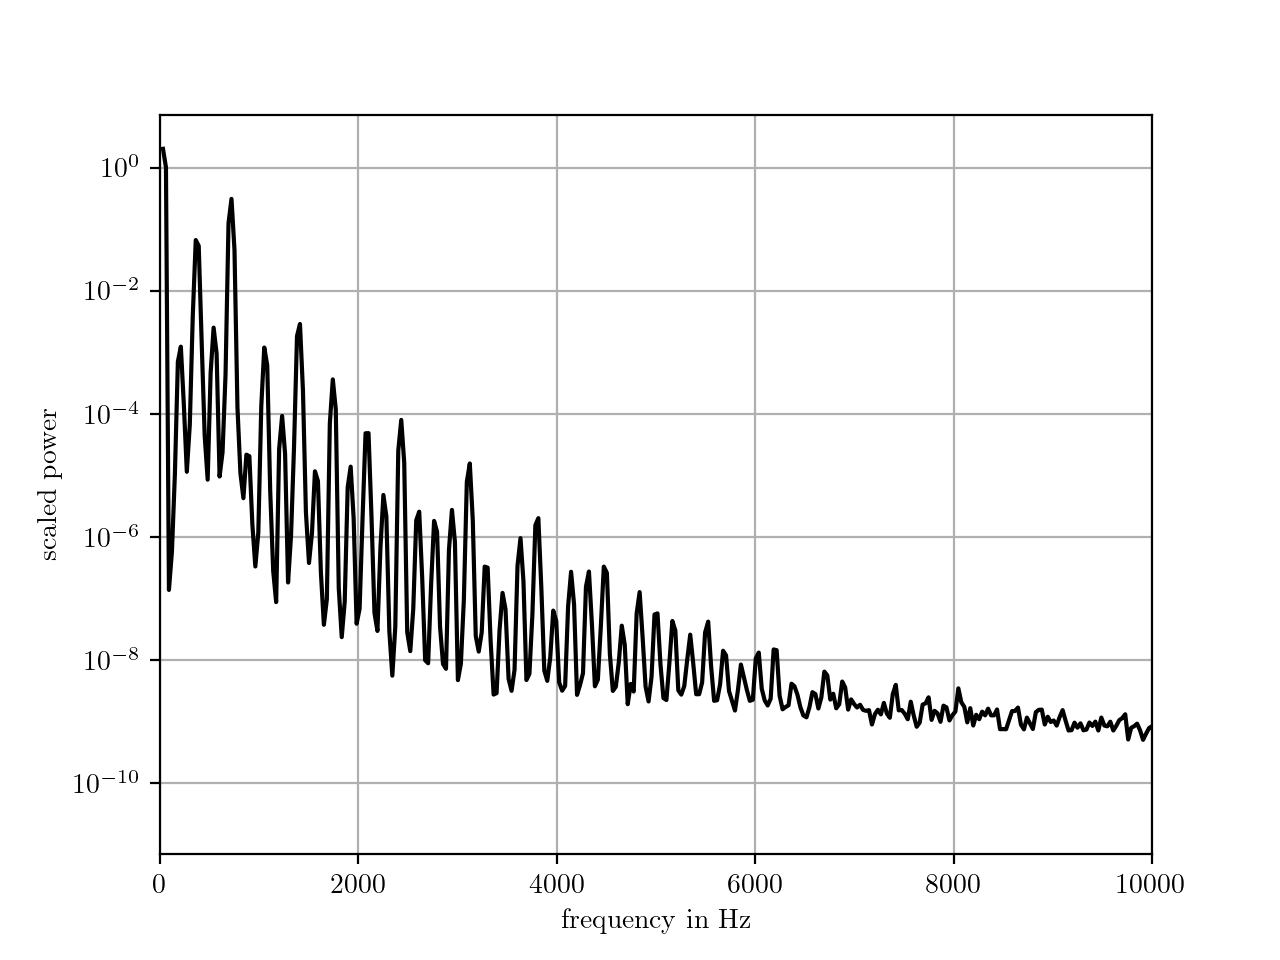
\includegraphics[width=\textwidth]{AuswPaul/Aufg-b/LS66.png}
        \caption{Leistungsspektrum}
    \end{subfigure}
    \caption{$R_1 = 66$ k$\Omega$}
    \label{fig:A66}
\end{figure}

Eine weitere Bifurkation findet im Übergang zu $R_1 = 66$ k$\Omega$ (Abbildung \ref{fig:A66}) statt. Was wiederum durch eine Zunahme an Peaks im Leistungsspektrum begleitet wird. Nun ist eine subharmonische Schwingung mit $\frac{1}{4} f_0$ zu erkennen. Ein Blick auf den Attraktor bestätigt das sich der Oszillator nun in Periode 4 befindet.
\newpage
\begin{figure}[h]
    \centering
    \begin{subfigure}[b]{0.45\textwidth}
        \centering
        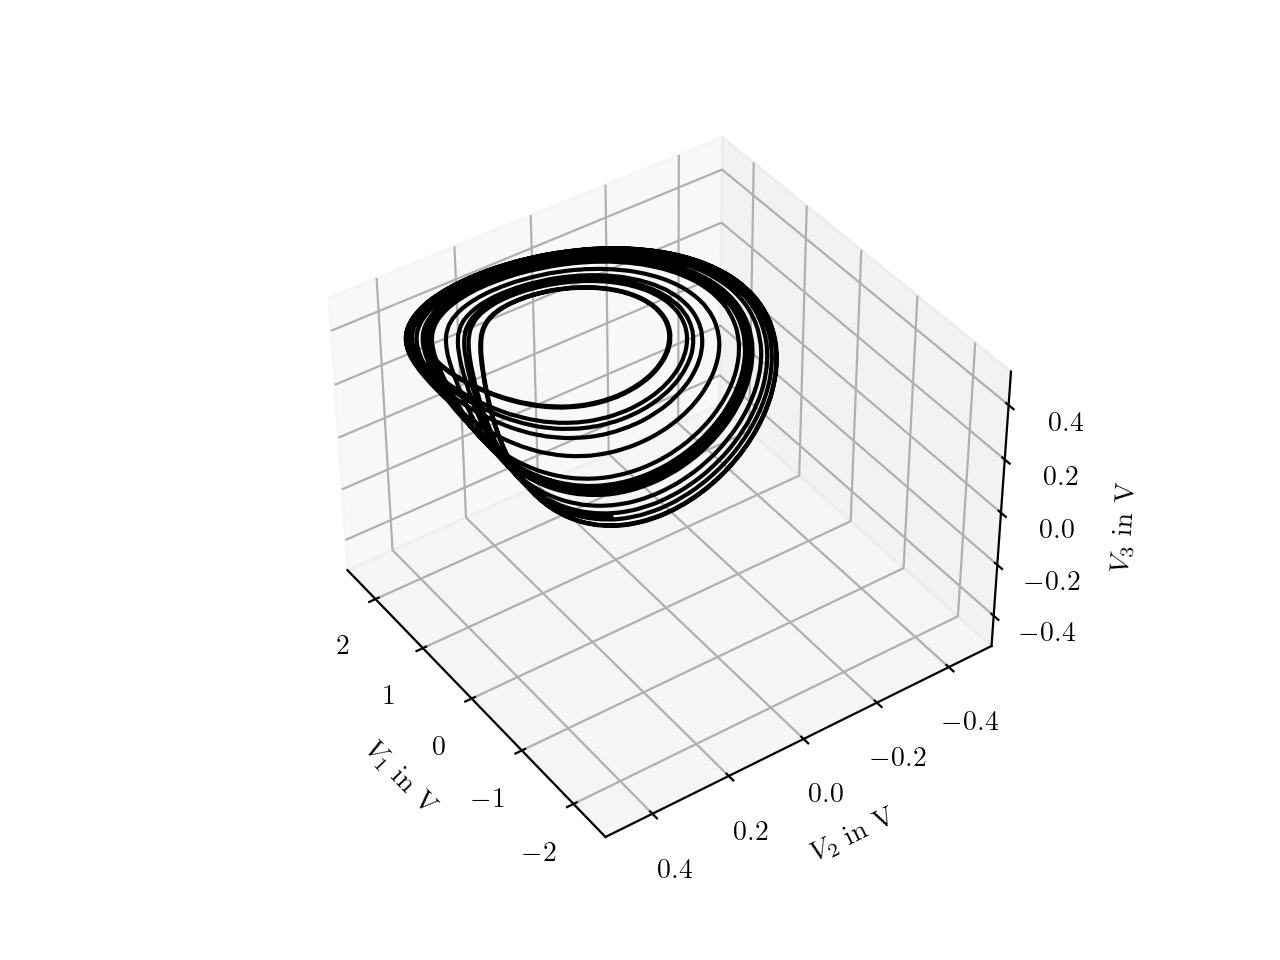
\includegraphics[width=\textwidth]{AuswPaul/Aufg-b/At70.png}
        \caption{Attraktor}
    \end{subfigure}
    \hfill
    \begin{subfigure}[b]{0.45\textwidth}
        \centering
        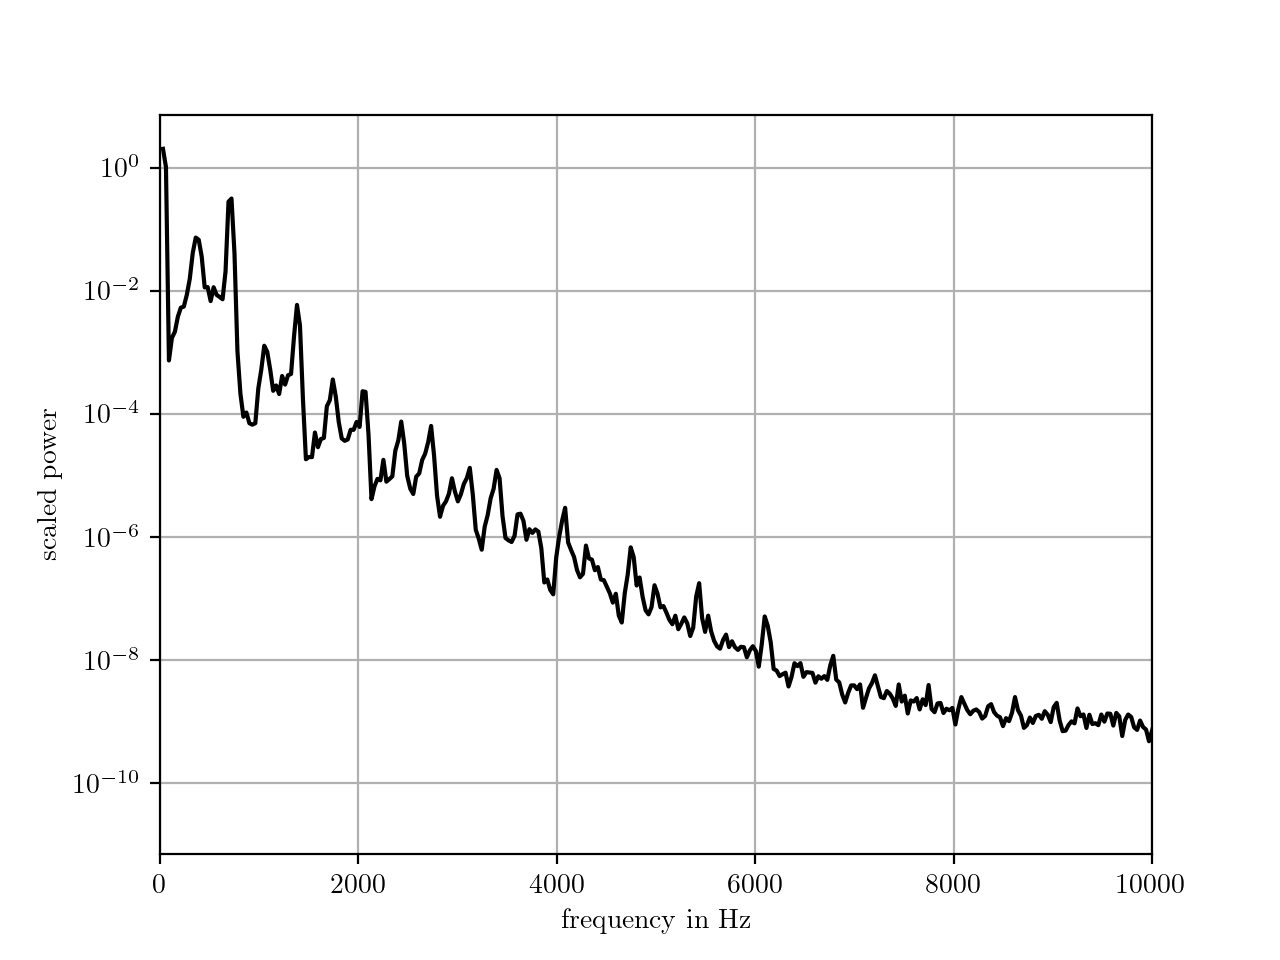
\includegraphics[width=\textwidth]{AuswPaul/Aufg-b/LS70.png}
        \caption{Leistungsspektrum}
    \end{subfigure}
    \caption{$R_1 = 70$ k$\Omega$}
    \label{fig:A70}
\end{figure}

Die nächste Phase zeigt nun zum ersten Mal chaotisches Verhalten, was sehr gut am nahezu kontinuierlich abnehmenden Leistungsspektrum und an dem Attraktor zu erkennen ist. Dies geschieht bei $R_1 = 70$ k$\Omega$ (Abbildung \ref{fig:A70}).

\begin{figure}[h]
    \centering
    \begin{subfigure}[b]{0.45\textwidth}
        \centering
        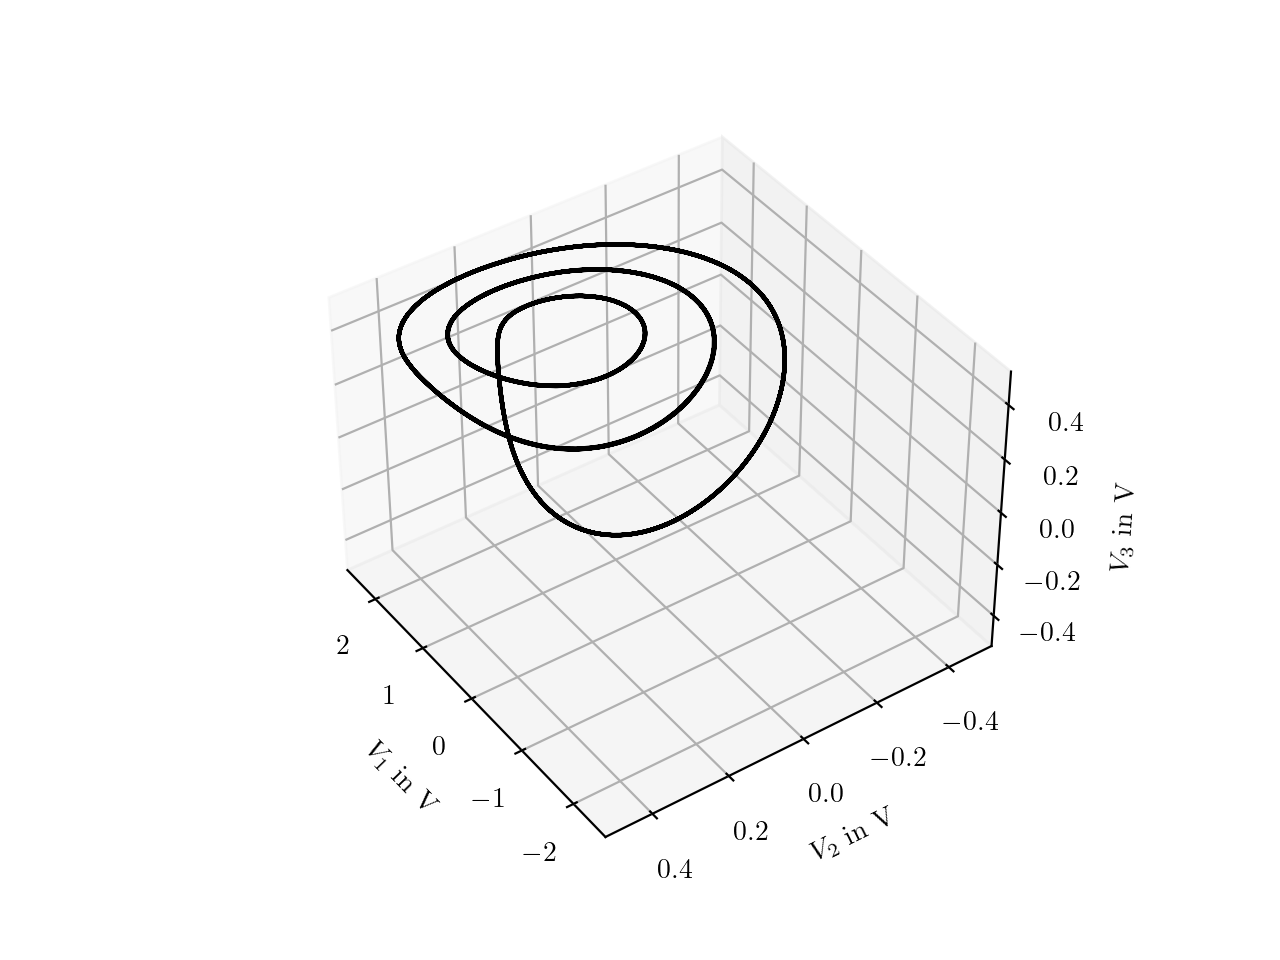
\includegraphics[width=\textwidth]{AuswPaul/Aufg-b/At73.png}
        \caption{Attraktor}
    \end{subfigure}
    \hfill
    \begin{subfigure}[b]{0.45\textwidth}
        \centering
        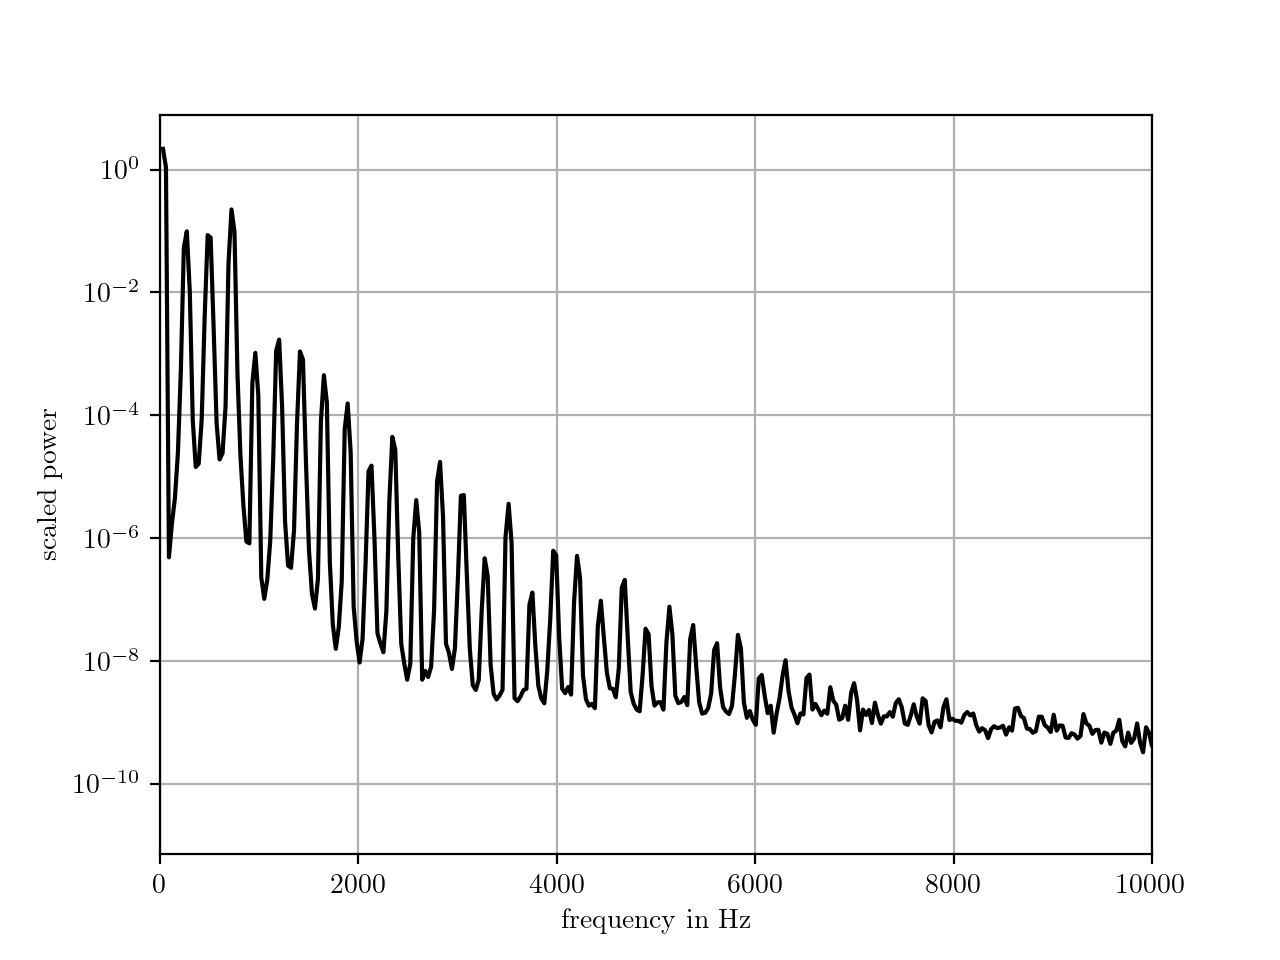
\includegraphics[width=\textwidth]{AuswPaul/Aufg-b/LS73.png}
        \caption{Leistungsspektrum}
    \end{subfigure}
    \caption{$R_1 = 73$ k$\Omega$}
    \label{fig:A73}
\end{figure}

Das Chaos wird durch ein Periode 3 Fenster durchbrochen, was der Plot des Attraktors bei $R_1 = 73$ k$\Omega$ (Abbildung \ref{fig:A73}) sehr gut verdeutlicht.

\begin{figure}[h]
    \centering
    \begin{subfigure}[b]{0.45\textwidth}
        \centering
        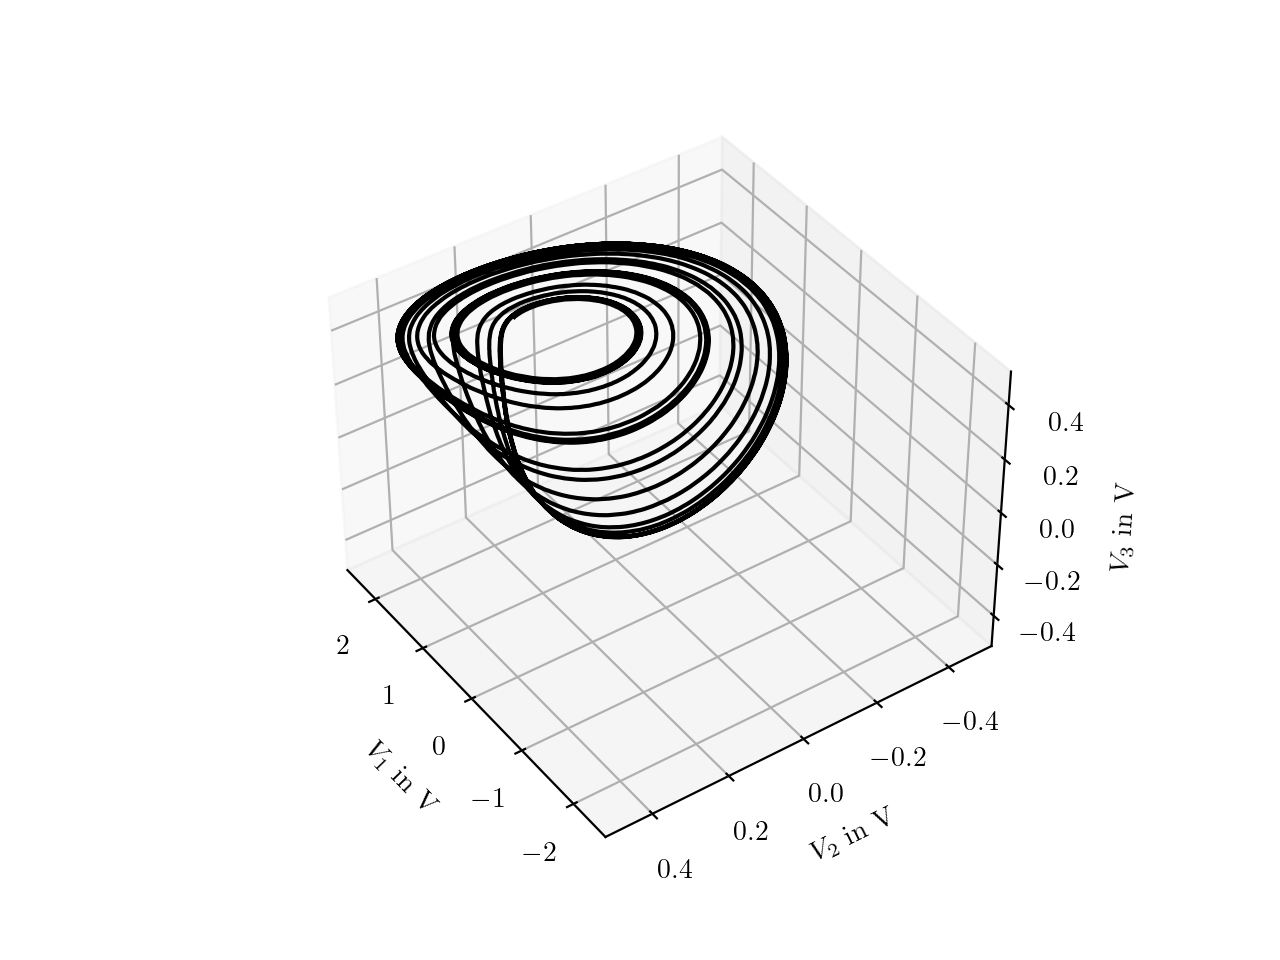
\includegraphics[width=\textwidth]{AuswPaul/Aufg-b/At74.png}
        \caption{Attraktor}
    \end{subfigure}
    \hfill
    \begin{subfigure}[b]{0.45\textwidth}
        \centering
        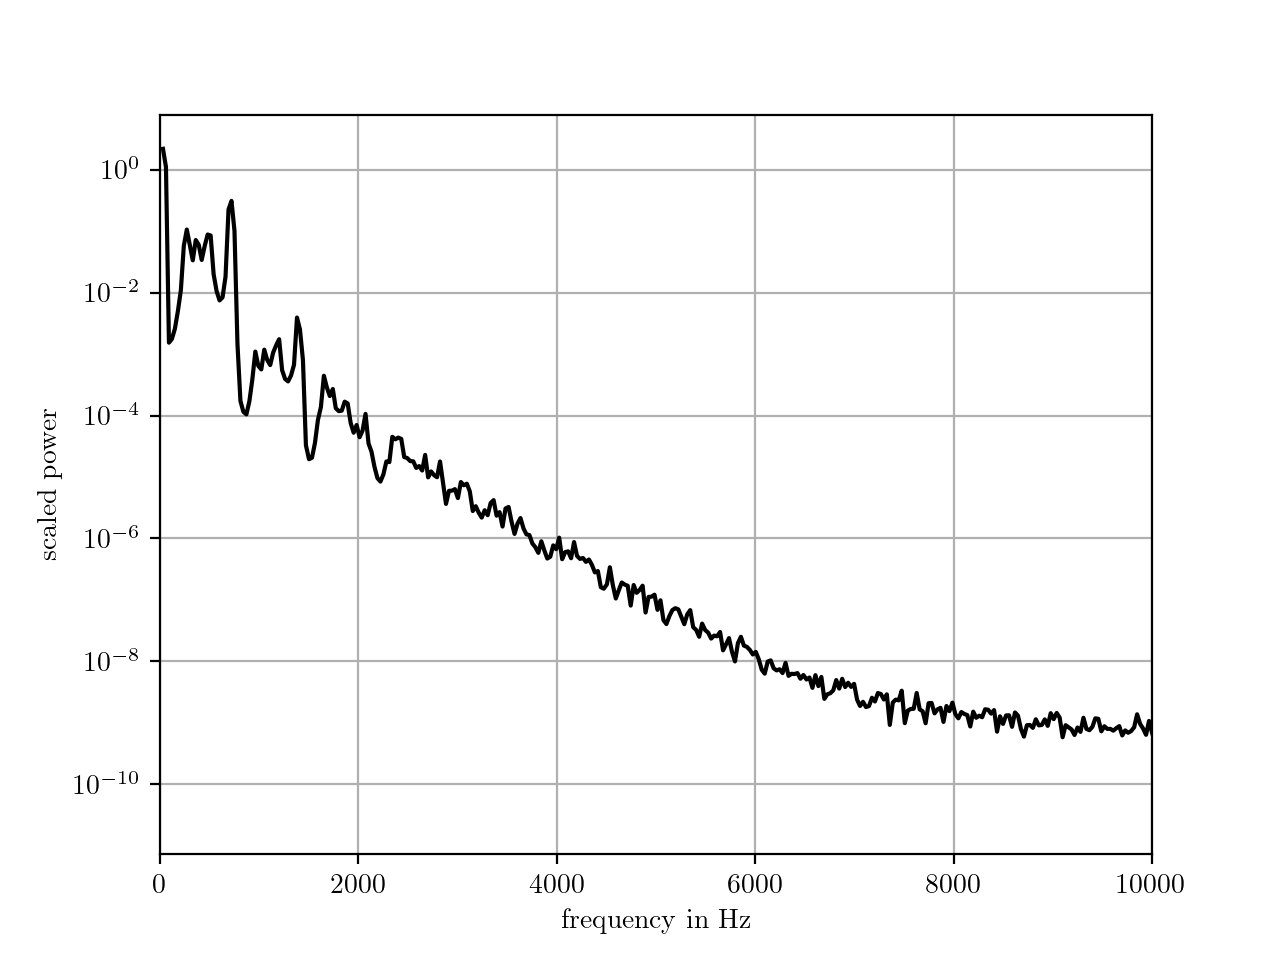
\includegraphics[width=\textwidth]{AuswPaul/Aufg-b/LS74.png}
        \caption{Leistungsspektrum}
    \end{subfigure}
    \caption{$R_1 = 74$ k$\Omega$}
    \label{fig:A74}
\end{figure}

\newpage
Anschließend bei $R_1 = 74$ k$\Omega$ (Abbildung \ref{fig:A74}) tritt, deutlich erkennbar, erneut Chaos auf.

\begin{figure}[h]
    \centering
    \begin{subfigure}[b]{0.45\textwidth}
        \centering
        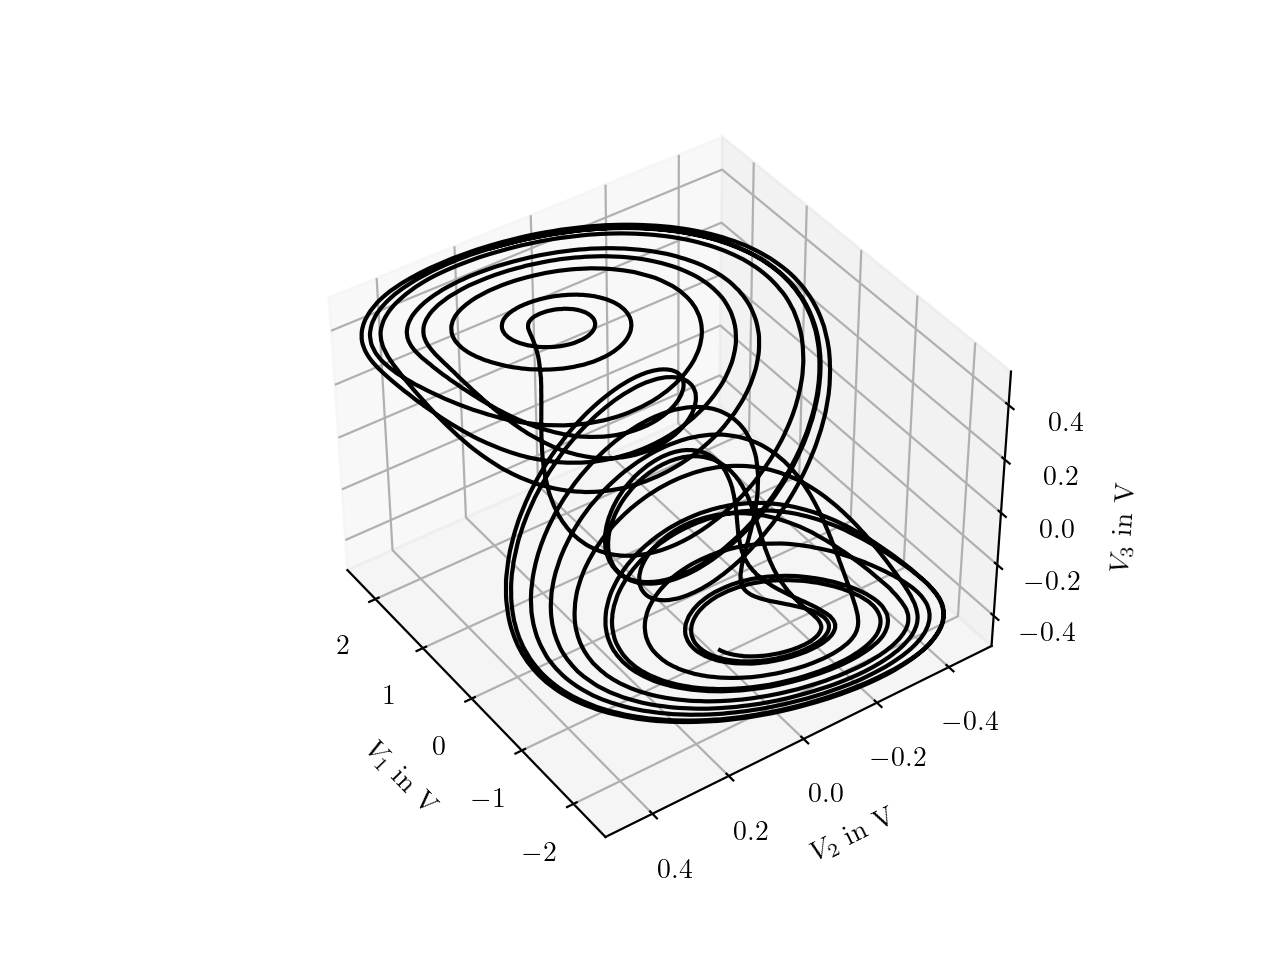
\includegraphics[width=\textwidth]{AuswPaul/Aufg-b/At100.png}
        \caption{Attraktor}
    \end{subfigure}
    \hfill
    \begin{subfigure}[b]{0.45\textwidth}
        \centering
        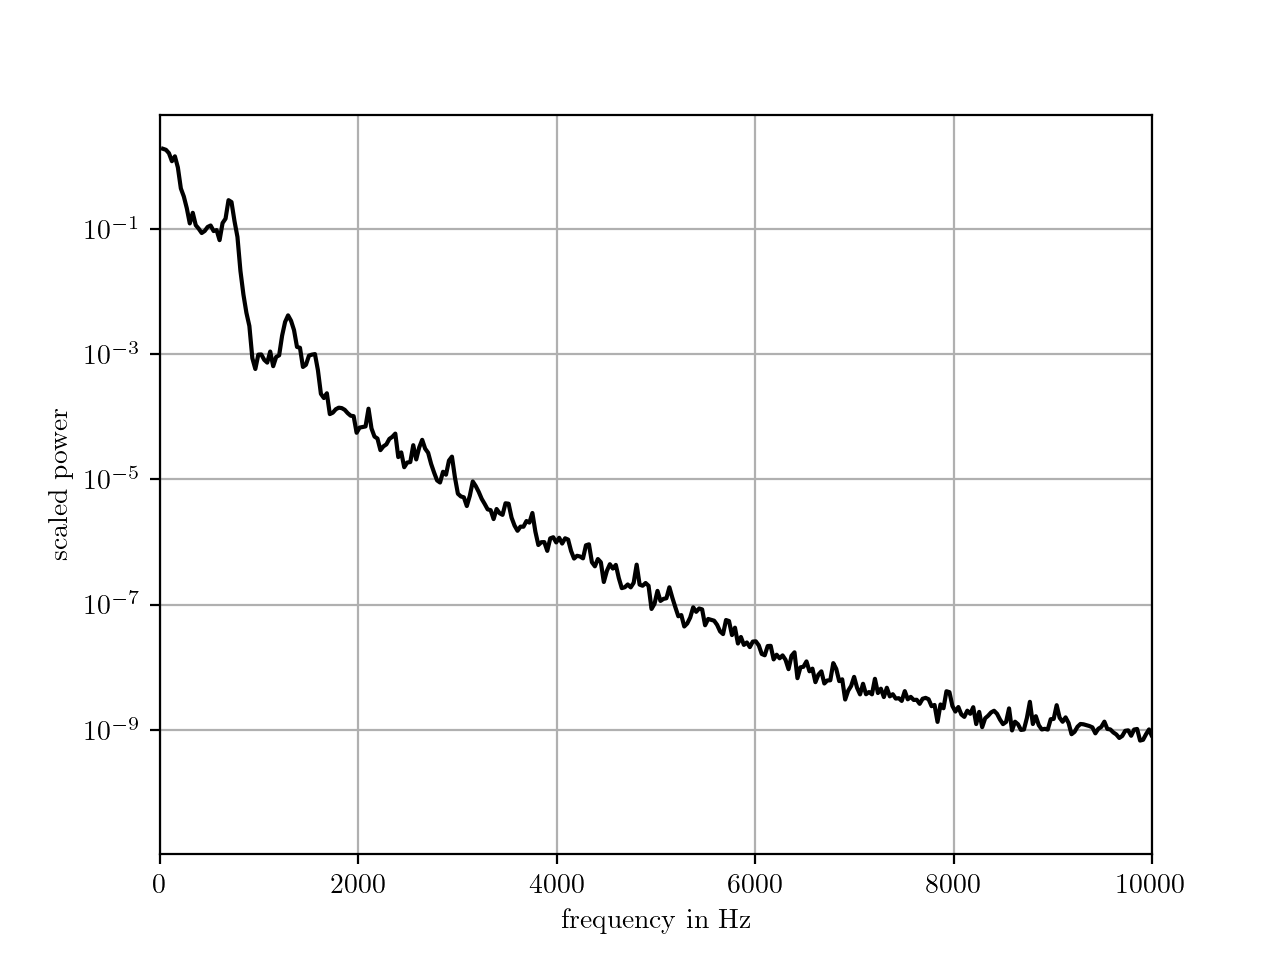
\includegraphics[width=\textwidth]{AuswPaul/Aufg-b/LS100.png}
        \caption{Leistungsspektrum}
    \end{subfigure}
    \caption{$R_1 = 100$ k$\Omega$}
    \label{fig:A100}
\end{figure}

Bei $R_1 = 100$ k$\Omega$ (Abbildung \ref{fig:A100}) ist das Double-scroll-chaos zu erkennen.
\newpage
\subsection{Bifurkationsdiagramm}
Um ein Bifurkationsdiagramm zu erstellen wurde ähnlich zum Schnitt durch das Phasendiagramm ein fester Wert (\(R_2=8,4k \Omega\)) eingestellt. Unter Zuhilfenahme des Labview Messprogramms konnte nun durch Variation von \(R_1\) folgendes Diagramm erstellt werden.

\begin{figure}[h]
    \centering
    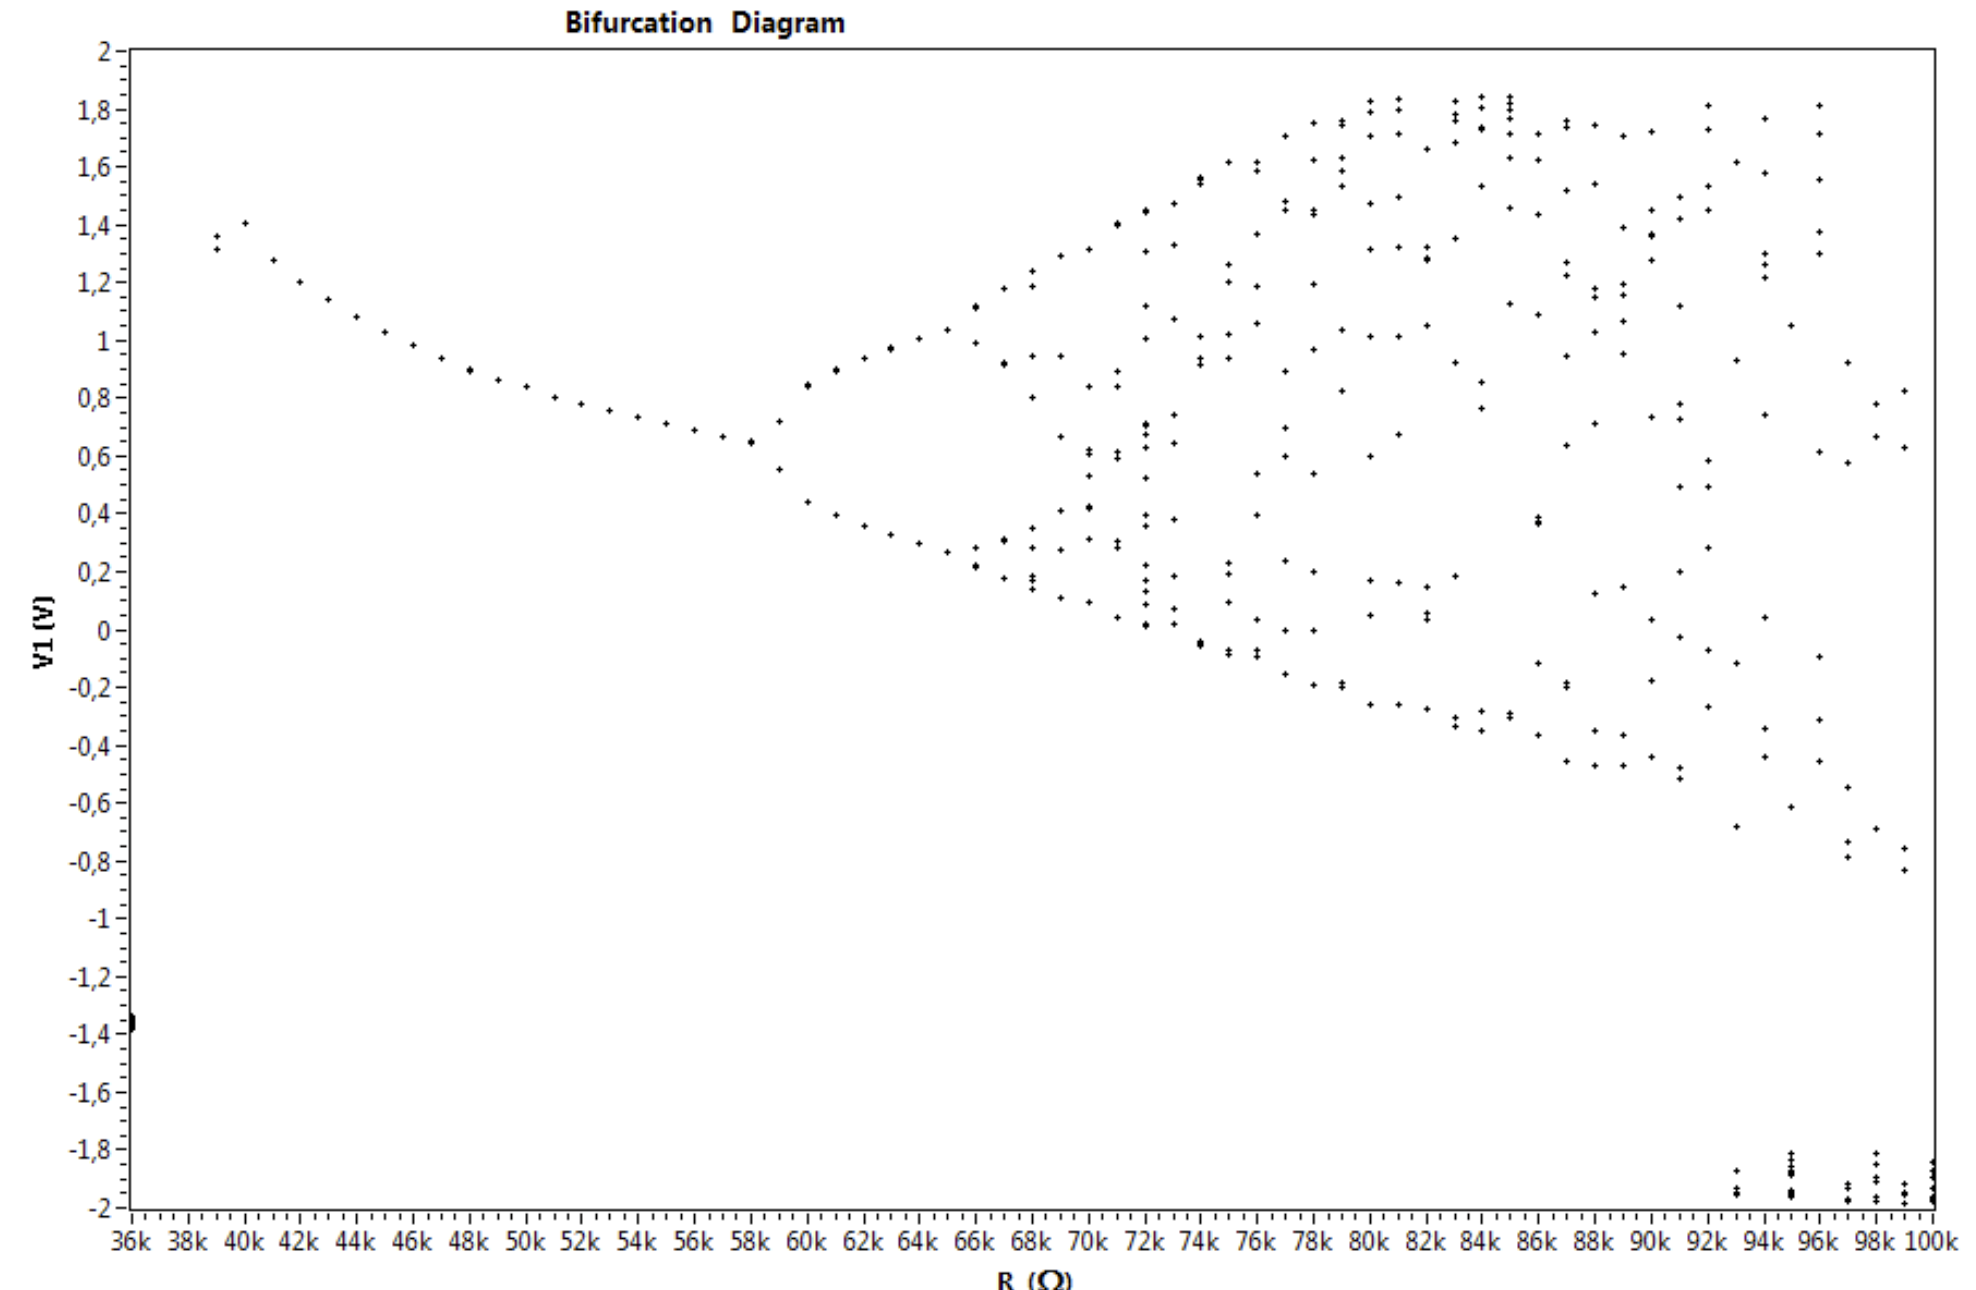
\includegraphics[width=\textwidth]{AuswPaul/BifurkDia.png}
    \caption{Bifurkationsdiagramm bei $R_2 = 8,4$ k$\Omega$ und variablen $R_1$}
\end{figure}

Im obigen Diagramm ist die erste Bifurkation (ca. $R = 58$ k$\Omega$) sehr deutlich zu erkennen aber auch die zweite (ca. $R = 66$ k$\Omega$) und dritte (ca. $R = 68$ k$\Omega$) sind noch zu erkennen. Ab ca. $R=93$ k$\Omega$ beginnt der Double-Scroll-Bereich. Leider ist bei der Messung der Fixpunktbereich etwas zu kurz gekommen, was wahrscheinlich der fortgeschritten Zeit und den damit einhergehenden Verlust der Konzentration zulasten zulegen ist. Außerdem würden mehr Messpunkte das Diagramm noch deutlicher machen.\\
Nun soll das Bifurkationsdiagramm mit der Simulation verglichen werden.

\newpage
\begin{figure}[h]
    \centering
    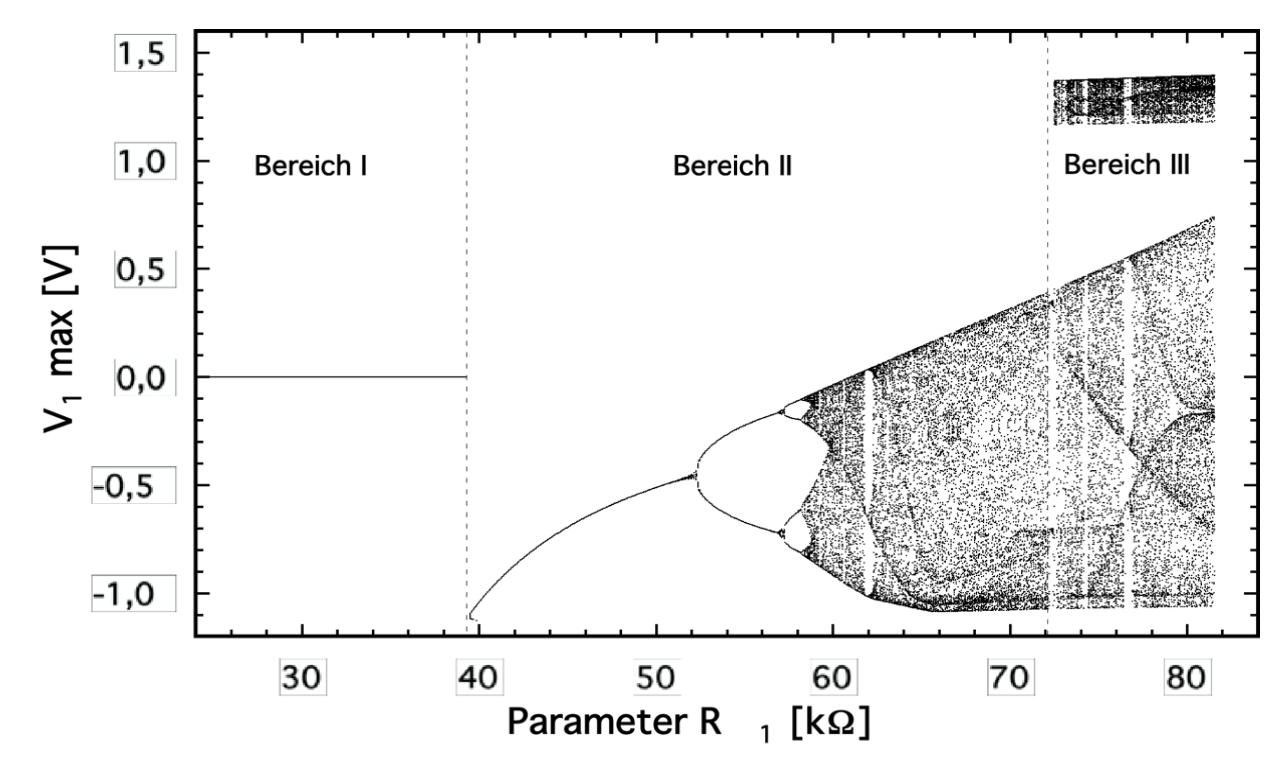
\includegraphics[width=\textwidth]{AuswPaul/BifuSim.png}
    \caption{Berechnetes Bifurkationsdiagramm (Abbildung 7 aus der Anleitung)}
\end{figure}

Betrachtet man die beiden Diagramme, so fällt auf, dass diese qualitativ gut übereinstimmen. Jedoch fällt auch auf, dass die Messung gegenüber der Simulation horizontal gespiegelt ist. Außerdem fallen auch Abweichungen auf. So ist die erste Bifurkation in der Messung bei ca. $R=58$ k$\Omega$ gegenüber $R=52$ k$\Omega$ in der Simulation verschoben.


\newpage
\subsection{Feigenbaum-Konstante}

Um die Feigenbaum-Konstante zu bestimmen wurden die Werte, bei denen eine Periodenverdopplung auftrat, ermittelt. 
Diese wurden durch eine separate Messung aufgenommen und nicht aus obigem Bifurkationsdiagramm abgelesen.
Damit wird versucht genauere Werte zu erhalten, da für das Bifurkationsdiagramm die Messdauer, im Vergleich zum direkten Suchen der Periodenverdopplungen, deutlich größer ist, ist es wahrscheinlicher, dass Störquellen, wie Temperaturveränderungen der Messgeräte, die Werte verfälschen.\\

Die Feigenbaum-Konstante \(\delta\) kann folgendermaßen berechnet werden: 
\begin{align}
    \delta = \lim_{n \to \infty} \delta_n \\
    \delta_n = \frac{r_n - r_{n-1}}{r_{n+1} -r_n}
\end{align}

Für den Fehler gilt: 
\begin{align}
    s_{\delta} = s_{R_1} \sqrt{ \left( \frac{1}{r_{n+1}-r_n}\right)^2 + \left(\frac{r_{n+1}-r_{n-1}}{(r_n - r_{n+1})^2}\right)^2 + \left(\frac{r_n - r_{n-1}}{(r_{n+1}-r_n)^2}\right)^2}\\
    \text{mit} \qquad s_{R_1} = 1 \, \text{k}\Omega
\end{align}

Der Literaturwert der Feigenbaum-Konstante ist: \(\delta = 4,6692...\)\\

Folgende Werte wurden gemessen: \\
\begin{tabular}{c c c}
    $r_1$ & $r_2$ & $r_3$\\
    \hline
    59 & 65,6 & 67,6
\end{tabular}

Mit unseren Werten ergibt sich: \(\delta_2 = (3 \pm 3)\)

Der Literaturwert liegt noch innerhalb des Fehlerintervalls. Eine Abweichung vom Literaturwert wäre allerdings nicht weiter erstaunlich, da die Feigenbaum-Konstante durch \( \delta = \lim_{n \to \infty} \delta_n\) gegeben ist. Für unseren Wert gilt jedoch \( n=2\).

\newpage
\subsection{Zum Einbettungstheorem}

% TODO #34
Im folgenden soll nun eine Attraktorrekonstruktion durchgeführtwerden.\\
Der Orginalattraktor wurde bei $R_1 = 51$ k$\Omega$ und $R_2 = 8,4$ k$\Omega$ aufgenommen.

\begin{figure}[h]
    \centering
    \begin{subfigure}[b]{0.45\textwidth}
        \centering
        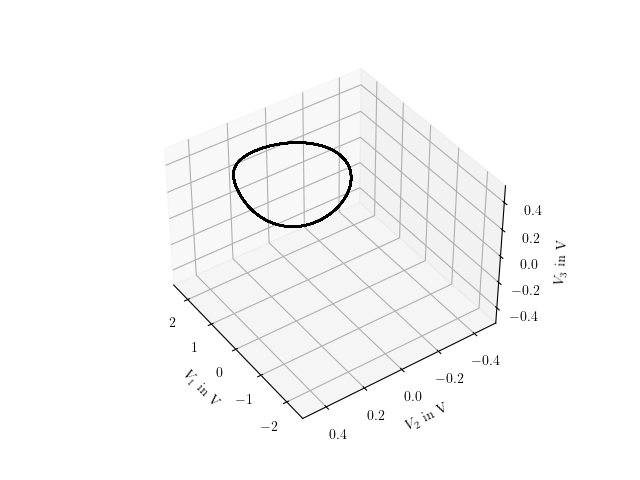
\includegraphics[width=\textwidth]{AuswPaul/Aufg-e/Attr.png}
        \caption{Attraktor}
    \end{subfigure}
    \hfill
    \begin{subfigure}[b]{0.45\textwidth}
        \centering
        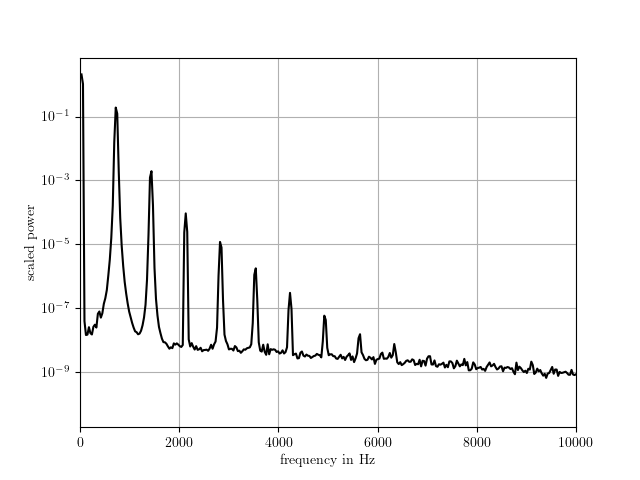
\includegraphics[width=\textwidth]{AuswPaul/Aufg-e/LS.png}
        \caption{Leistungsspektrum}
    \end{subfigure}
    \caption{$R_1 = 51$ k$\Omega$ und $R_2 = 8,4$ k$\Omega$}
\end{figure}

Die qualitativ beste Rekonstruktion wurde für den Verschiebungsindex $n= 60$ n erreicht.\\
Die Delayzeit kann mit folgender Formel berechnet werden: 
\begin{align}
    \tau = n \, \frac{1}{f_{abtast}} \qquad \text{mit} \quad f_{abtast} = 150 \, \text{kHz}
\end{align}
Somit gilt: $\tau = 0,4 \text{ms}$ \\

Der größte Peak aus dem Leistungsspektrum liegt bei $f=724$ Hz, da der nächst kleinere nur noch ein $\frac{1}{10}$ davon hat kann er bei der Ermittlung der mittleren Umlaufdauer vernachlässigt werden. Somit gilt für die mittlere Umlaufdauer: 
\begin{align}
    \bar{T} = \frac{1}{724} = 1,38 \, \text{ms}
\end{align}
Vergleicht man die beiden Werte, so fällt auf, dass sie sich in etwa der gleichen Größenordnung bewegen.
\begin{align}
    \frac{\bar{T}}{\tau} = 3,45 \Rightarrow \tau \approx \frac{\bar{T}}{4}
\end{align}

\newpage
Außerdem soll die Rekonstruktion noch für einen chaotischen Attraktor durchgeführt werden. Der Orginalattraktor wurde bei $R_1 = 70$ k$\Omega$ und $R_2 = 8,4$ k$\Omega$ aufgenommen, wie in Abbildung \ref{fig:A70E} zu sehen.
\begin{figure}[h]
    \centering
    \begin{subfigure}[b]{0.45\textwidth}
        \centering
        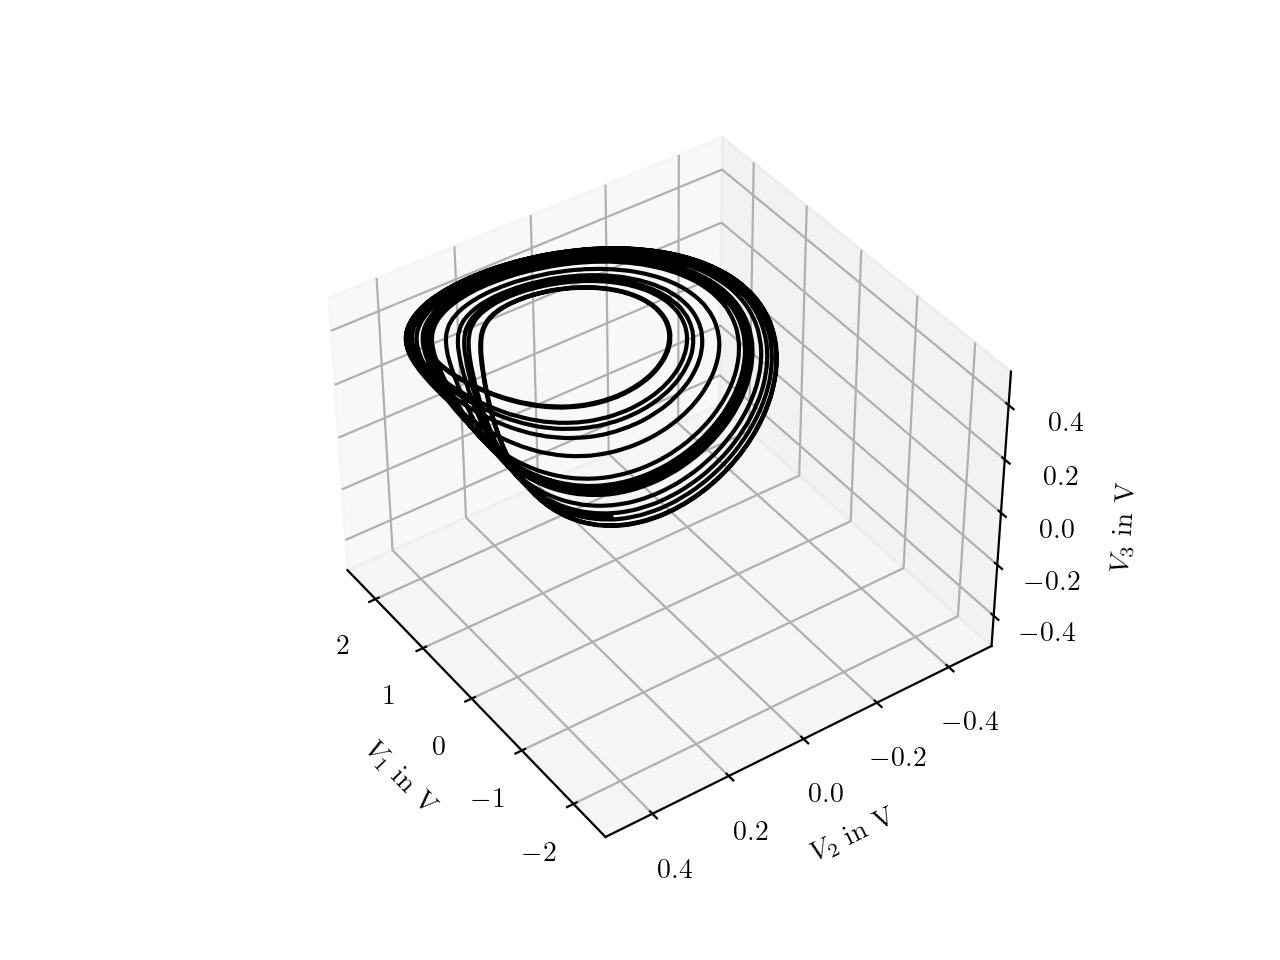
\includegraphics[width=\textwidth]{AuswPaul/Aufg-b/At70.png}
        \caption{Attraktor}
    \end{subfigure}
    \hfill
    \begin{subfigure}[b]{0.45\textwidth}
        \centering
        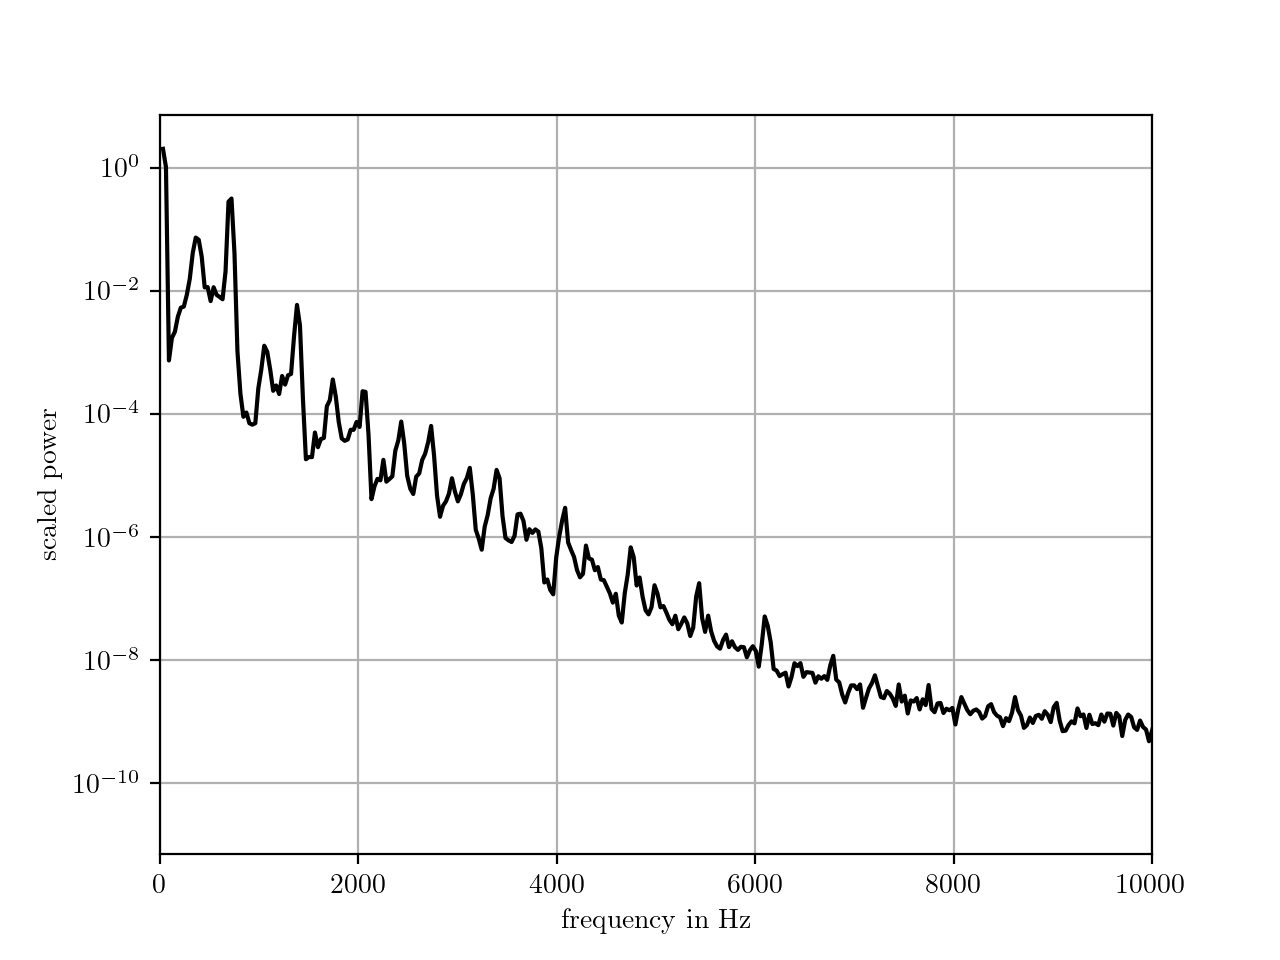
\includegraphics[width=\textwidth]{AuswPaul/Aufg-b/LS70.png}
        \caption{Leistungsspektrum}
    \end{subfigure}
    \caption{$R_1 = 70$ k$\Omega$}
    \label{fig:A70E}
\end{figure}

Mit Hilfe eines selbst geschriebenen Pythonskripts wurde nun das beste $n$ für die Attraktorrekonstruktion ermittelt. Das Ergebnis ist in Abbildung \ref{fig:AR70} zu sehen.

\begin{figure}[h]
    \centering
    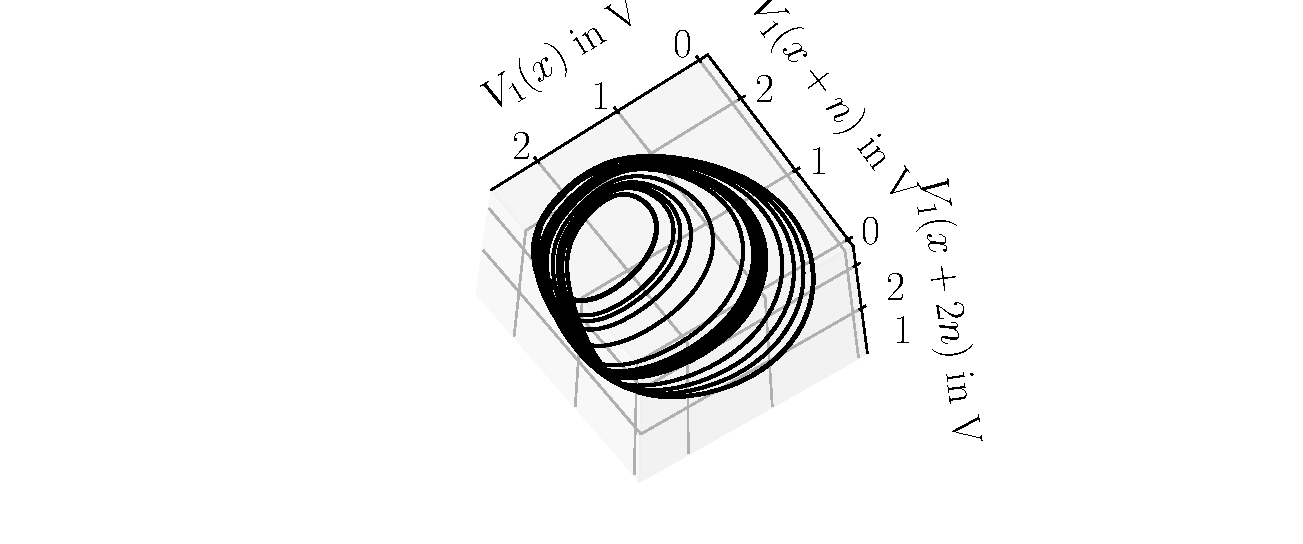
\includegraphics[width=\textwidth]{AuswPaul/Aufg-e/AR70.pdf}
    \caption{Attraktorrekonstruktion für $n=44$}
    \label{fig:AR70}
\end{figure}

Genau wie oben wird das Verhältnis der beiden zahlen gebildet:
\begin{align}
    \tau = n \, \frac{1}{f_{abtast}} \qquad \text{mit} \quad f_{abtast} = 150 \, \text{kHz}
\end{align}
Somit gilt: $\tau = 0,3 \text{ms}$ \\
\begin{align}
    \bar{T} = \frac{1}{730} = 1,37 \, \text{ms}
\end{align}
\begin{align}
    \frac{\bar{T}}{\tau} = 4,6  \Rightarrow \tau \approx \frac{\bar{T}}{4}
\end{align}
Es fällt auf, dass das Verhältnis nahe $\frac{1}{4}$ liegt.